% ++++++++++++++++++++++++++++++++++++++++
% Don't modify this section unless you know what you're doing!
\documentclass[letterpaper,12pt]{article}
\usepackage{tabularx} % extra features for tabular environment
\usepackage{amsmath}  % improve math presentation
\usepackage{graphicx} % takes care of graphic including machinery
\usepackage[margin=0.75in,letterpaper]{geometry} % decreases margins
\usepackage{cite} % takes care of citations
\usepackage[final]{hyperref} % adds hyper links inside the generated pdf file
\usepackage{listings}
\usepackage{csvsimple}
\usepackage{verbatim}
\usepackage{float}
\usepackage{graphicx} % Allows including images
\hypersetup{
	colorlinks=true,       % false: boxed links; true: colored links
	linkcolor=black,        % color of internal links
	citecolor=blue,        % color of links to bibliography
	filecolor=magenta,     % color of file links
	urlcolor=blue         
}
%++++++++++++++++++++++++++++++++++++++++
\setlength{\parindent}{0pt}
\setlength\parskip{1em plus 0.1em minus 0.2em}

\begin{document}
\title{%
Electron Spin Resonance \\
\large PHY224 Lab 6}
\author{Fredrik Dahl Bråten, Pankaj Patil}
\date{\today}
\maketitle
%\tableofcontents
%\listoffigures
%\listoftables

\section{Abstract}

In this exercise we experimentally calculate the gyromagnetic ratio $\gamma$ for an electron. 
As we expect the ratio to be greater than the theoretically predicted value of $e/2m$, 
we compute this discrepancy in terms of \emph{Lande g factor}. This analysis was done in Python by use of the numpy, scipy and matplotlib modules.

\section{Introduction}

The potential energy acquired by an electron in presence of external magnetic field $\vec{B}$ is given by
$$E = -\vec{\mu} \cdot \vec{B}$$
Where, $\mu$ is magnetic dipole moment of the electron.

The relationship between magnetic moment and the spin angular momentum of the electron is given by,
$$\vec{\mu} = \gamma \vec{S}$$

Where $\gamma$ is gyromagnetic ratio. 

For ideal electron, we expect $\gamma$ to be equal to $e/2m$. But for real world electron, it it greater than $e/2m$.
This discrepancy is given by \emph{Lande g Factor}, which is defined as
$$g = \frac{\gamma}{e/2m} > 1$$
If an electron absorbs photon with energy equal to the difference between the two spin energy level, then 
it can flip it's orientation. This phenomenon is called \emph{Electron Spin Resonance}. 

The energy difference between the two spin levels is given by,
$$\Delta E = \gamma \hbar B_z$$
Where, $B_z$ is the uniform z-component of the external magnetic field. By equating above with energy of a photon $h\nu$, we get
$$\nu = \frac{1}{2\pi}\gamma B_z$$
Now in the experimental setup the external magnetic field is generated by the two Helmholtz coils. The magnetic field produced
by the coils is given by,
$$B_z = \left(\frac{4}{5}\right)^\frac{3}{2} \frac{\mu_0 n I}{R}\ Tesla$$
Where,
\begin{itemize}
  \item[] $\mu_0 = 4\pi \times 10^{-7}\ N/A^2$
  \item[] $n$ = number of turns = 320
  \item[] $I$ = current through thee coils
  \item[] $R$ = the radius of the coils     
\end{itemize}

By measuring the current using the oscilloscope, we compute the magnetic field produced by the coils. Using the frequency counter, we note down the
resonance frequency. With these values we can use the relationship between $\nu$ and $B_z$ to compute $\gamma$ and hence the 
\emph{Lande g Factor}. For the computation of the magnetic field, we used half the measured value of the current, as the current is split between 
the two identical coils.

\section{Methods, Materials and Experimental Procedure}

We successfully followed the procedures as described by the TA and lab manual \cite{lab-manual-ex6} for this experiment.

\section{Results}

From our model of Frequency vs Magnetic field we found the linear relationship between the two is given 
by 
$$f(B) = m\nu$$
Where,
\begin{itemize}
  \item[] $B$ = External Magnetic Field in Tesla
  \item[] $\nu$ = Resonance Frequency in $MHz$
  \item[] $m$ = Slope of the linear curve 
\end{itemize}

This relation is plotted in following graph,

\begin{figure}[H]
  \centering
  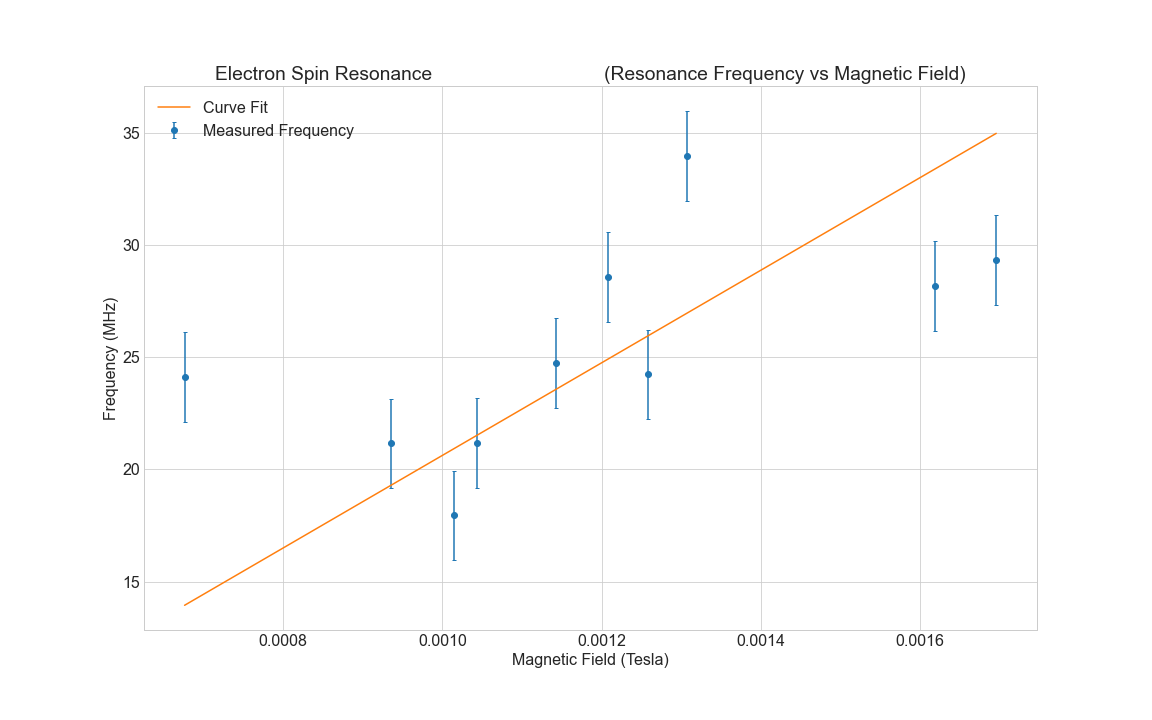
\includegraphics[width=0.95\linewidth]{../code/Pankaj/lab6_freq_vs_magnetic_field.png}    
  \begin{center}
    \begin{center}
      Model Function : $f(x) = mx$ \\
      Slope $m = 21471.7312\ T/MHz$\\
      $\chi_{red}^2 = 8.2622$
    \end{center}  \end{center}
  \caption{Frequency vs Magnetic Field}
  \label{frq-vs-b}
\end{figure}

After the data analysis using Python, we found 
\begin{itemize}
  \item[] $m$ = 21471.7312 $T/MHz$
  \item[] Gyromagnetic Ratio $\gamma = 134910.87 \pm 2450.10\ rad/s/T$
  \item[] Lande $g$ Factor = 1.53 $\pm$ 0.03
  \item[] $\chi_{red}^2 = 8.2622$ 
\end{itemize}

Using the measured currents, which give us the measured external magnetic field, 
and the measured resonance frequency, we obtained \emph{Lande g Factor} for each measurement.
These factors for each frequency is plotted in following graph. The standard deviation
of the \emph{Lande g Factors} is used for the error bars in the graph.

\begin{figure}[H]
  \centering
  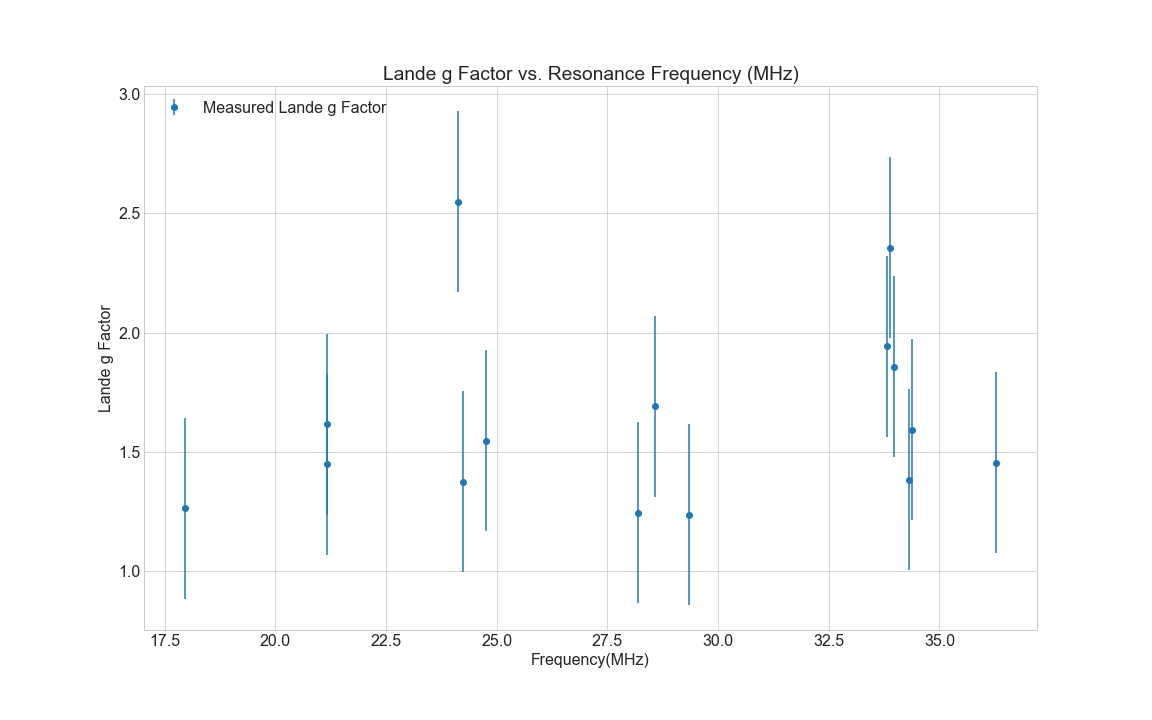
\includegraphics[width=1.0\linewidth]{../code/Pankaj/lab6_g_factor_vs_freq.png}    
  \begin{center}
    \begin{center}   
    \end{center}  \end{center}
  \caption{Lande g Factor vs Frequency}
  \label{lande-vs-frq}
\end{figure}

\section{Discussion}

For the linear model without the y-intercept, we found the linear fit with $\chi_{red}^2 = 8.2622$. As this value 
is in order of magnitude 1, we can say that the linear fit is a good fit. 

From the Figure \ref{frq-vs-b}, it is clear that not all the data points are close to the linear fit. These large 
deviations can be attributed to sensitivity of the instruments, and also large uncertainty in the measurements.

We observed that the copper coils used to put electron in precision have lot of impact on the data. The data points 
are closer to the line for the copper coil with highest number of turns. For medium number of turns, the 
data points are further away from the linear fit. We did not get any good measurement for the copper coil with lowest
number of turns. It was difficult to achieve precise resonance frequency for the coil with lowest number of turns.

We observed very high uncertainty (2 $MHz$) in the measurement of resonance frequency.

Now we answer the questions asked in the manual,

\textbf{Question 1}
The measuring signal through the basic unit reaches the output Y with a time delay relative to 
the magnetic field applied. Hence there is a phase shift in the two signals we measure in the 
oscilloscope, giving us the asymmetry for the ESR signal about the maximum current point. 

\textbf{Question 2}
The relation from equation (8) in the manual is true over a wide range of frequencies and the relation is linear. 
This is because $E=h\nu$ for light of every frequency. Furthermore, the energy gap between the spin up and spin down states of an electron is always $\Delta E = \gamma  \hbar  B_z$.

\textbf{Question 3}
The width of the peak can be attributed to electrons having energies spread because of their velocity distribution and/or because of the spin interactions between them. 
Because of the this spread, $\Delta E$ is also spread over these velocity distribution, and hence  we observe slightly different
absorption frequencies for this spread, giving the absorption lines some width. 

\textbf{Question 4}
When the resonance condition is matched, i.e. when the $\Delta E = \gamma \hbar B_z$, the electrons 
in the sample absorb this energy, and  the oscillating circuit is loaded. As a result impedance of the
oscillating circuit changes, and voltage at the copper coil decreases. This voltage is converted into 
measuring signal. This is how the basic unit for this experiment works. 

The voltage converted to measuring signal is fed out of the Y socket. 

The knob that adjusts the frequency is connected to the Frequency counter, which has multiple 1/1000. That is why 
we multiply the frequency readings by 1000 to obtain actual resonance frequency.

\section{Conclusions}
In this exercise we studied the Electron Spin Resonance phenomenon. Using the uniform external magnetic 
field, we observe the variation of resonance frequency with respect to the current through the Helmholtz coils
producing the magnetic field. As predicted by theory, we observe the relationship is linear, and the linear
fit to the measured data was found to be in order of magnitude 1. Using the linear model fit, we 
computed the gyromagnetic ratio $\gamma$ and the \emph{Lande g Factor}. Again as predicted by the theory 
the value of \emph{Lande g Factor} was found to be greater than 1.


\pagebreak

\appendix

\section{Appendix}

\subsection{Oscilloscope Readings}

\begin{figure}[H]
  \centering
  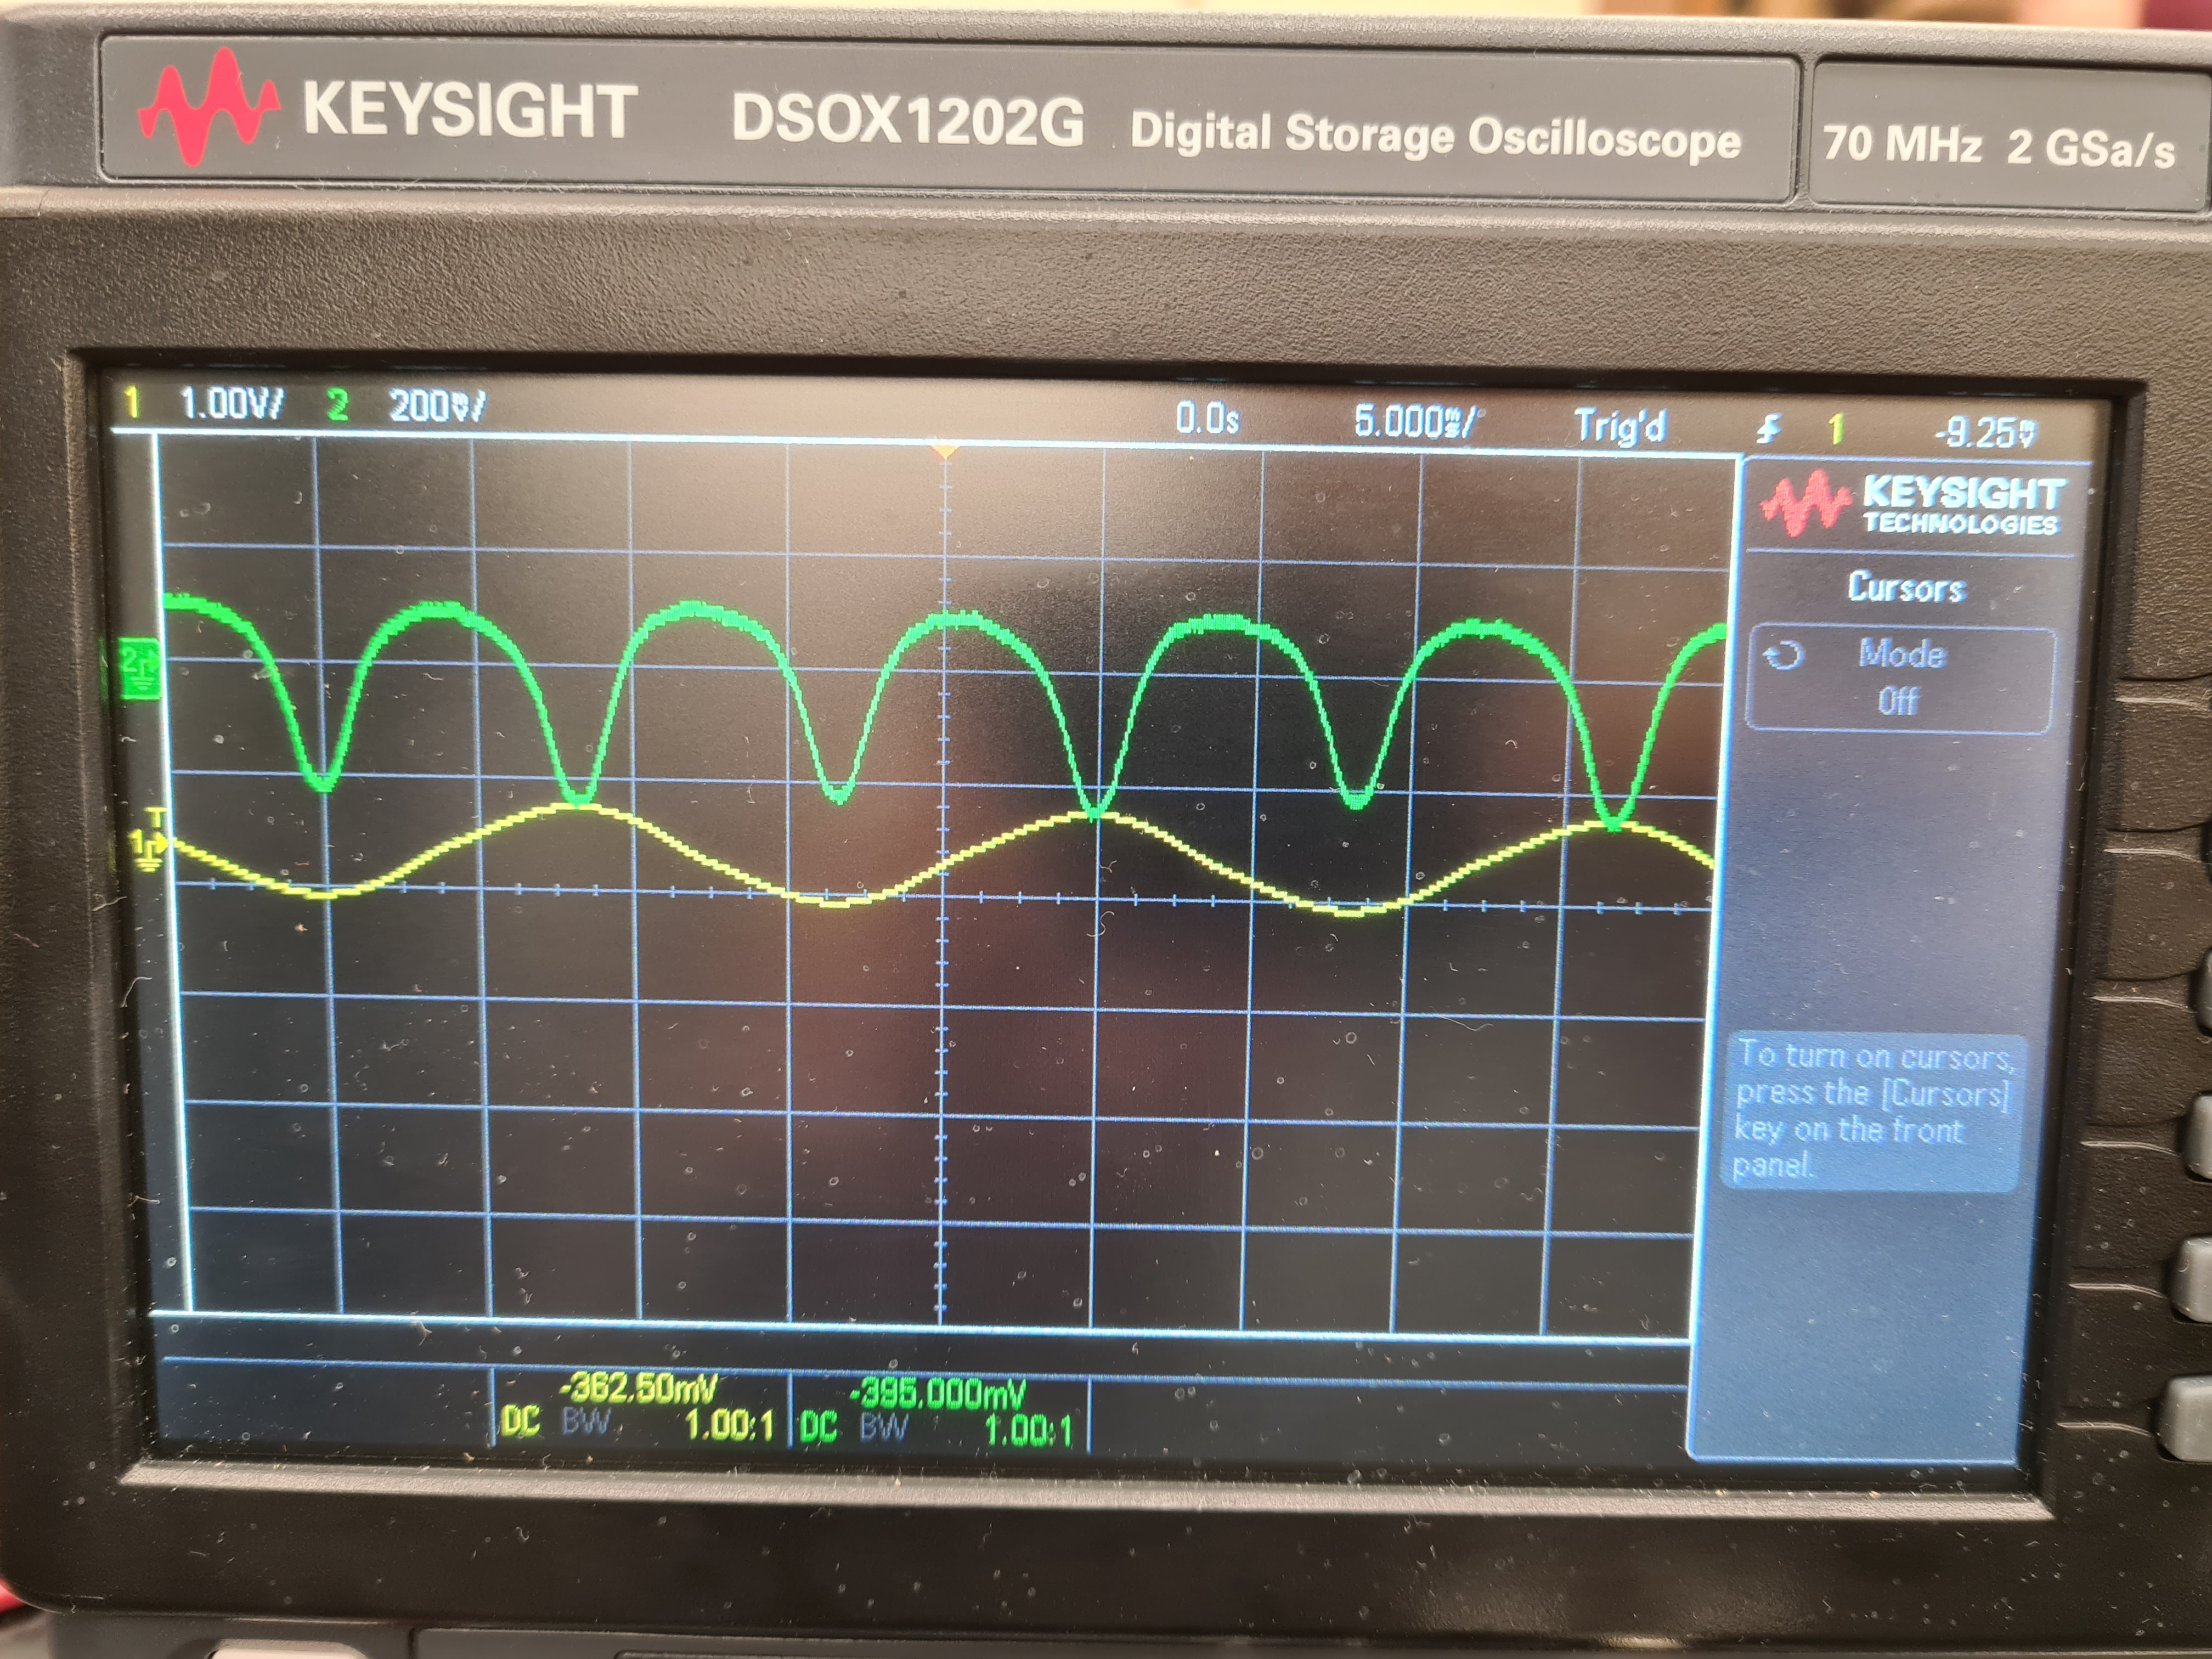
\includegraphics[width=1.0\linewidth]{../Fredrik/osc-p-p.jpg}    
  \begin{center}
    \begin{center}   
    \end{center}  \end{center}
  \caption{Oscilloscope Reading (Peak to Peak Alignment)}
  \label{osc}
\end{figure}

\begin{figure}[H]
  \centering
  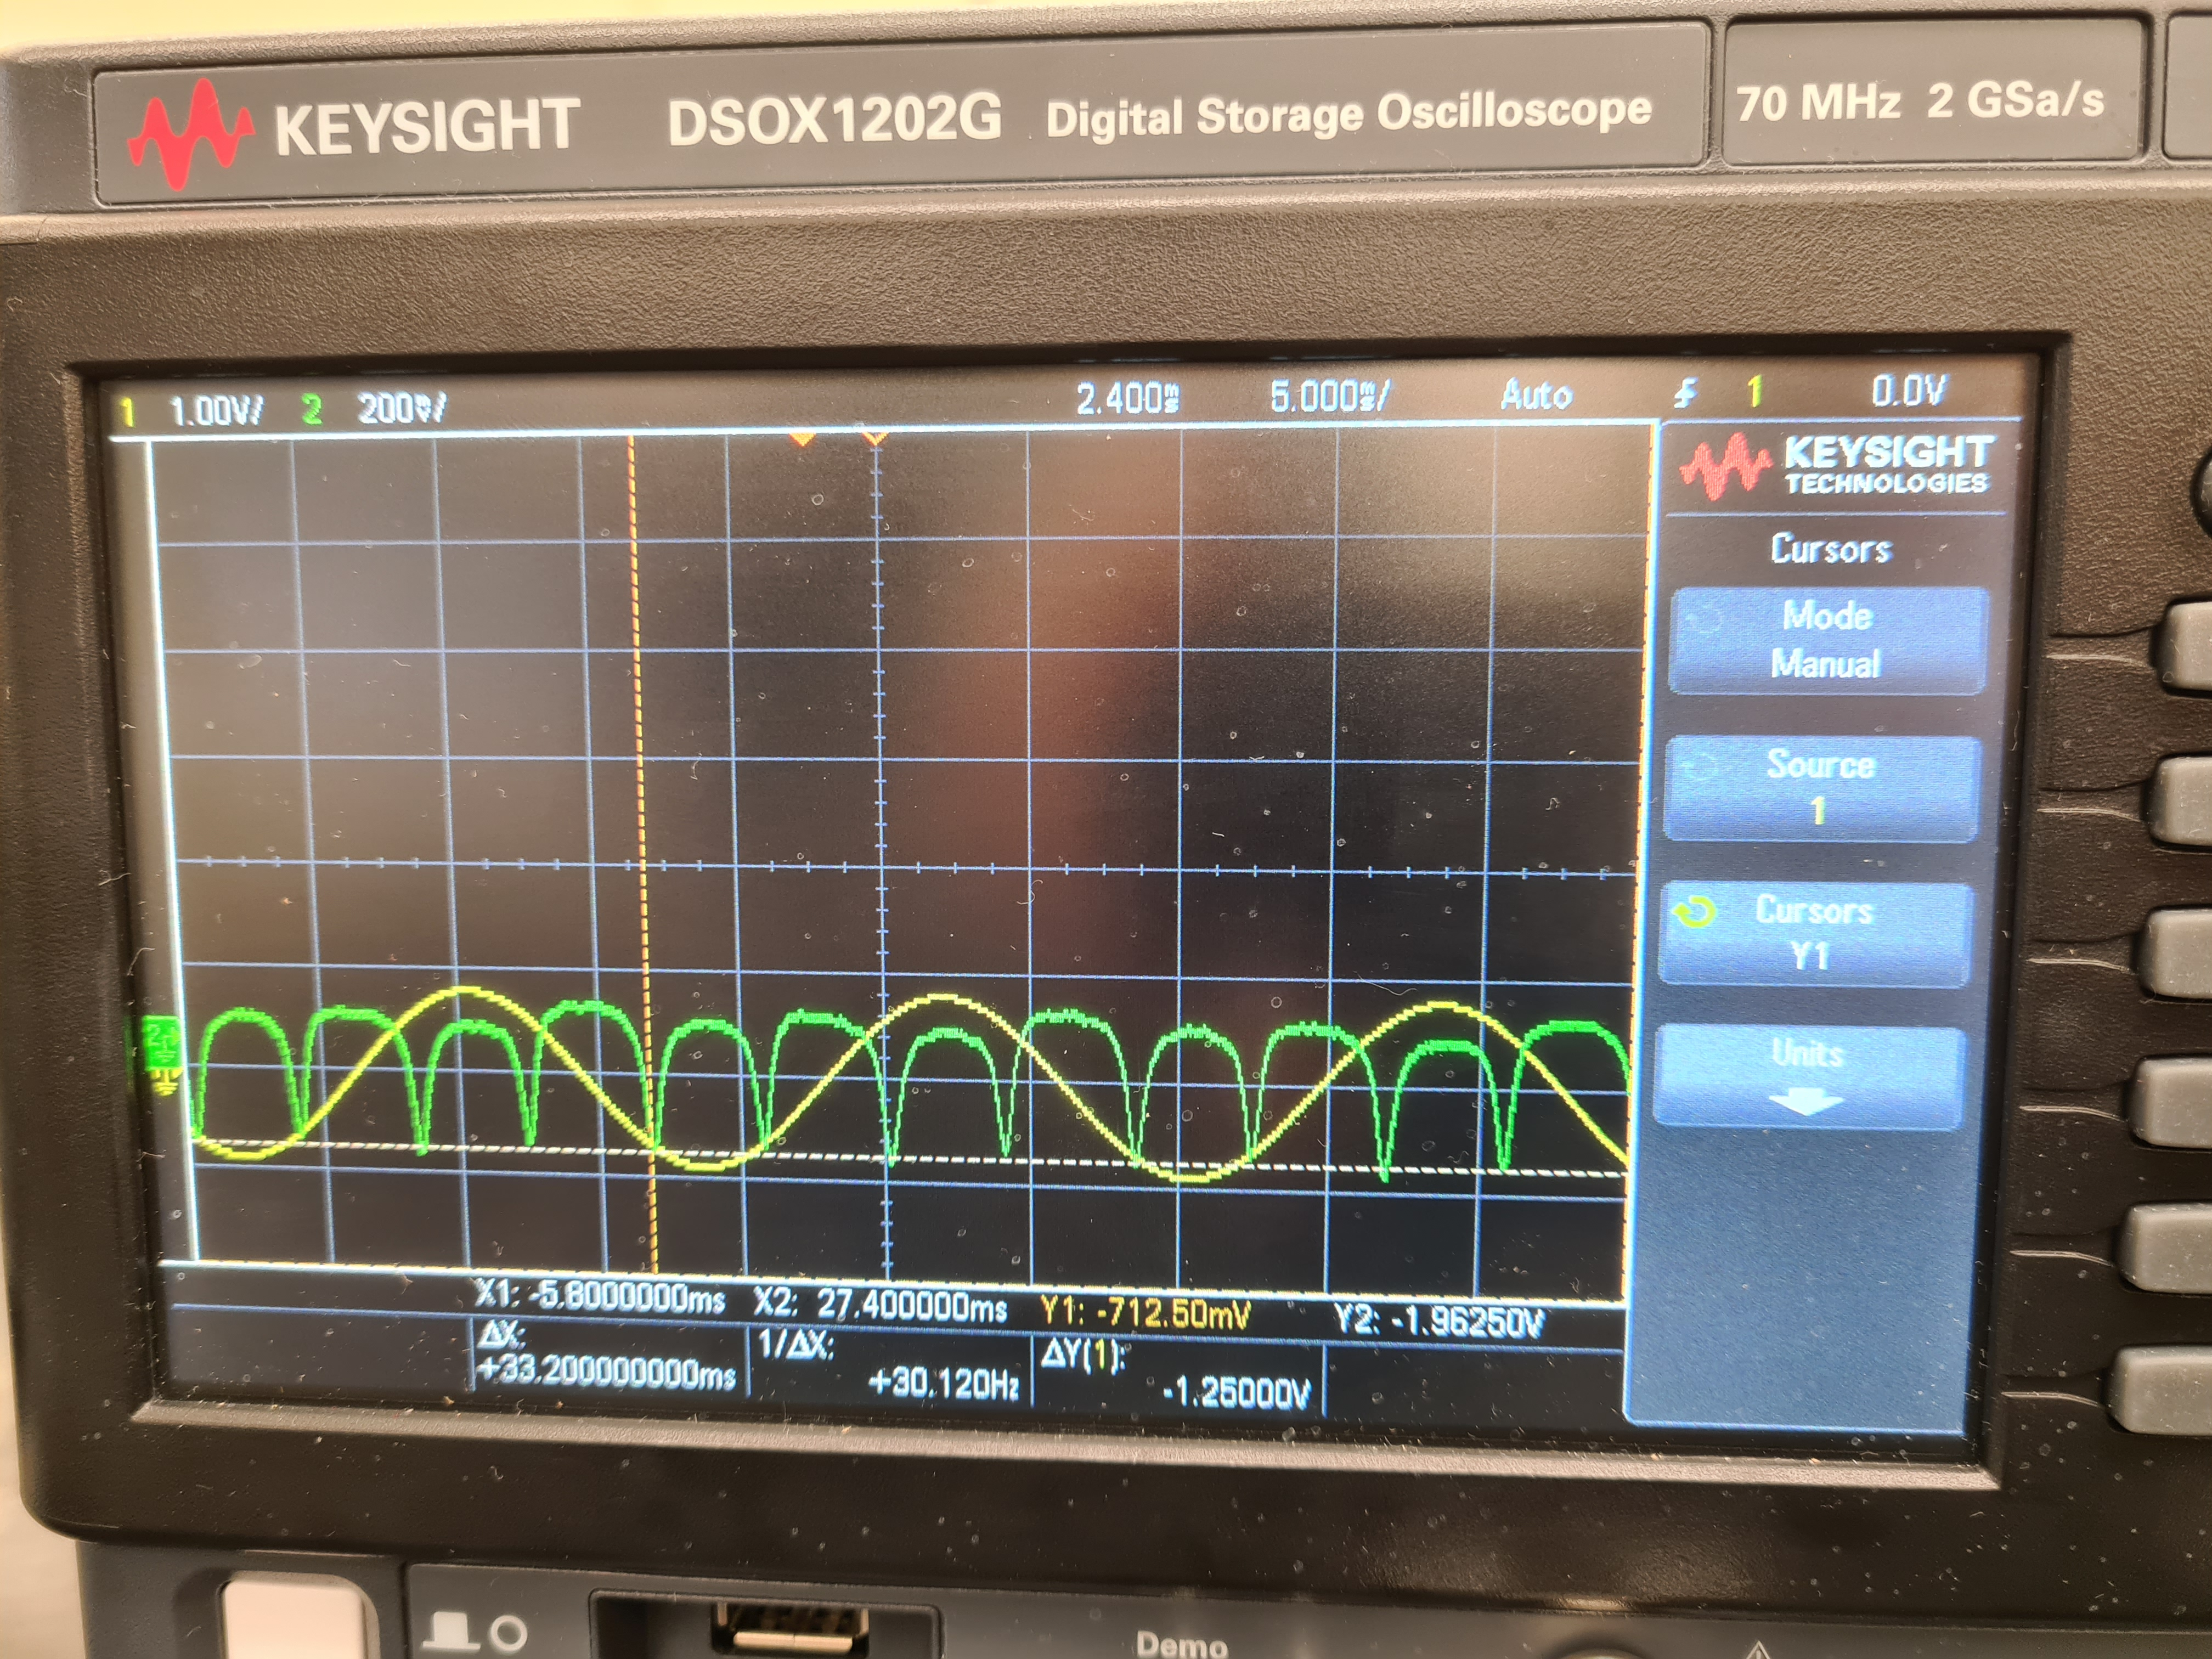
\includegraphics[width=1.0\linewidth]{../Fredrik/osc-p-not-aligned.jpg}    
  \begin{center}
    \begin{center}   
    \end{center}  \end{center}
  \caption{Oscilloscope Reading (Peaks Not Aligned)}
  \label{osc}
\end{figure}

\pagebreak

\subsection{Python Code}

The Python code for this exercise is divided into two files. statslab.py file contains utility methods
which we will be frequently using in this course. lab\_6.py file contains the code which analyzes
the data.

\subsubsection{statslab.py}
\noindent\rule{\textwidth}{1pt}
\verbatiminput{../code/Pankaj/statslab.py}
\noindent\rule{\textwidth}{1pt}

\pagebreak

\subsubsection{lab\_6.py}
\noindent\rule{\textwidth}{1pt}
\verbatiminput{../code/Pankaj/lab_6.py}
\noindent\rule{\textwidth}{1pt}

\pagebreak

\begin{thebibliography}{99}

\bibitem{lab-manual-ex6} Electron Spin Resonance - electric-spin.pdf.pdf

\end{thebibliography}

\end{document}
